\documentclass[10pt, landscape]{article}
\usepackage[scaled=0.92]{helvet}
\usepackage{calc}
\usepackage{multicol}
\usepackage{ifthen}
\usepackage[a4paper,margin=3mm,landscape]{geometry}
\usepackage{amsmath,amsthm,amsfonts,amssymb}
\usepackage{color,graphicx,overpic}
\usepackage{hyperref}
\usepackage{newtxtext} 
\usepackage{enumitem}
\usepackage{amssymb}
\usepackage[table]{xcolor}
\usepackage{vwcol}
\usepackage{tikz}
\usetikzlibrary{arrows.meta}
\usetikzlibrary{calc}
\usepackage{mathtools}
\usepackage{nicematrix}
%For pictures / figures
\usepackage{color,graphicx,overpic}
\graphicspath{ {./images/} }
% for relations
\usepackage{cancel}
\usepackage{ mathrsfs }
\graphicspath{ {./images/} }
\setlist{nosep}


\pdfinfo{
  /Title (CG1111A-Quiz2.pdf)
  /Creator (TeX)
  /Producer (pdfTeX 1.40.0)
  /Author (Seamus)
  /Subject (Example)
  /Keywords (pdflatex, latex,pdftex,tex)}

% Turn off header and footer
\pagestyle{empty}

\newenvironment{tightcenter}{%
  \setlength\topsep{0pt}
  \setlength\parskip{0pt}
  \begin{center}
}{%
  \end{center}
}

% redefine section commands to use less space
\makeatletter
\renewcommand{\section}{\@startsection{section}{1}{0mm}%
                                {-1ex plus -.5ex minus -.2ex}%
                                {0.5ex plus .2ex}%x
                                {\normalfont\large\bfseries}}
\renewcommand{\subsection}{\@startsection{subsection}{2}{0mm}%
                                {-1explus -.5ex minus -.2ex}%
                                {0.5ex plus .2ex}%
                                {\normalfont\normalsize\bfseries}}
\renewcommand{\subsubsection}{\@startsection{subsubsection}{3}{0mm}%
                                {-1ex plus -.5ex minus -.2ex}%
                                {1ex plus .2ex}%
                                {\normalfont\small\bfseries}}%
\renewcommand{\familydefault}{\sfdefault}
\renewcommand\rmdefault{\sfdefault}
% makes nested numbering (e.g. 1.1.1, 1.1.2, etc)
\renewcommand{\labelenumii}{\theenumii}
\renewcommand{\theenumii}{\theenumi.\arabic{enumii}.}
\renewcommand\labelitemii{•}
%  for logical not operator
\renewcommand{\lnot}{\mathord{\sim}}
\renewcommand{\bf}[1]{\textbf{#1}}
\newcommand{\abs}[1]{\vert #1 \vert}
\newcommand{\Mod}[1]{\ \mathrm{mod}\ #1}

\makeatother
\definecolor{myblue}{cmyk}{1,.72,0,.38}
\everymath\expandafter{\the\everymath \color{myblue}}
% Define BibTeX command
\def\BibTeX{{\rm B\kern-.05em{\sc i\kern-.025em b}\kern-.08em
    T\kern-.1667em\lower.7ex\hbox{E}\kern-.125emX}}
\let\iff\leftrightarrow
\let\Iff\Leftrightarrow
\let\then\rightarrow
\let\Then\Rightarrow

% Don't print section numbers
\setcounter{secnumdepth}{0}

\setlength{\parindent}{0pt}
\setlength{\parskip}{0pt plus 0.5ex}
%% this changes all items (enumerate and itemize)
\setlength{\leftmargini}{0.5cm}
\setlength{\leftmarginii}{0.5cm}
\setlist[itemize,1]{leftmargin=2mm,labelindent=1mm,labelsep=1mm}
\setlist[itemize,2]{leftmargin=4mm,labelindent=1mm,labelsep=1mm}

%My Environments
\newtheorem{example}[section]{Example}
% -----------------------------------------------------------------------

\begin{document}
\raggedright
\footnotesize
\begin{multicols}{4}


% multicol parameters
% These lengths are set only within the two main columns
\setlength{\columnseprule}{0.25pt}
\setlength{\premulticols}{1pt}
\setlength{\postmulticols}{1pt}
\setlength{\multicolsep}{1pt}
\setlength{\columnsep}{2pt}

\begin{center}
    \fbox{%
        \parbox{0.8\linewidth}{\centering \textcolor{black}{
            {\Large\textbf{CS2030S Final}}
            \\ \normalsize{AY24/25 sem 2}}
            \\ {\footnotesize \textcolor{myblue}{github.com/mendax1234}} 
        }%
    }
\end{center}

\section{First Half}
\begin{enumerate}
    \item \textbf{Information Hiding}:
    \begin{itemize}
        \item \textbf{fields} should be declared as \texttt{private}
        \item \textbf{methods} should be declared as \texttt{public}
    \end{itemize}
    \item \textbf{\texttt{final}}: \texttt{final} in a \textbf{method declaration} prevents \textbf{overriding}.
    \item \textbf{Heap and Stack}
    \begin{itemize}
        \item \textbf{Stack}: Stack contains stack frames, which are created whenever a \textbf{method} is called. It contains (\textbf{From bottom to up})
        \begin{itemize}
            \item the \texttt{this} reference (If \textbf{instance method} is called)
            \item the method arguments
            \item local variables within the method.
        \end{itemize}
        \item \textbf{Heap}: Contains the following (\textbf{From up to bottom}):
        \begin{itemize}
            \item \textbf{Class name}. (If a \textbf{lambda expression}, then write the expression)
            \item Instance fields and respective fields.
            \item Captured values. (Separated by \textbf{dashed lines})
        \end{itemize}
    \end{itemize}
    \item \textbf{Override vs. Overload}
    \begin{itemize}
        \item \textbf{Override}: must have \textbf{same method descriptor (method signature + method return type)}, e.g.\texttt{A C::foo(B1,B2)}, (B1, B2 are the type of the method parameters, same for as follows)
        \item \textbf{Overload}: must have same \textbf{method name}, in the same class and \textbf{different method signature (method name, number of parameters, type of each parameter, order of the parameters)}. e.g. \texttt{C::foo(B1,B2)}. \textbf{The return type of the method doesn't matter.}
    \end{itemize}
    \item \textbf{Tell, Don't Ask}: We never \textbf{ask} an object to spit out its own \textbf{raw data}. Instead, we \textbf{let the object know} what we want so that it can give us a piece of \textbf{processed data} (via an instance method).
    \begin{itemize}
        \item \textbf{Sample reasoning}: The subclass should ask the super class to do the thing (to be changed).
    \end{itemize}
    \item \textbf{Liskov Substitution Principle}: A \textit{subclass} \textbf{should not} break the expectations / \textbf{specifications} set by the \textbf{superclass}. \textbf{Tips}:
    \begin{itemize}
        \item Always write down what the specifications are set by the superclass.
        \item Construct a method and test whether the subclass can be substituted without breaking the specifications. (If class B \textbf{extends} A, and \textbf{overrides} the method in A, then \textbf{successful substitution} means \textbf{when substitute A with B}, we should call the \textbf{overridden function in B}!)
    \end{itemize}
    \item \textbf{Method Invocation}: Pay attention to the \textbf{CTT, RTT} of the \textbf{target} and the \textbf{CTT} of the \textbf{parameter}. The \textbf{RTT} of the \textbf{parameter} doesn't matter!
    \begin{itemize}
        \item During the compile time, find the \textbf{most specific} method descriptor starting from the CTT of the target. (Method M is \textbf{more specific than} method N means that the \textbf{type of the parameter of M} is the \textbf{subtype} of the \textbf{type of the parameter in N}).
        \item During the run time, use the method descriptor we got from above to find \textbf{the first} method from the \texttt{RTT} to \texttt{Object} and execute it.
        \item \textbf{Type casting} happens during the \textbf{compile tile}! e.g. \texttt{(Circle) o2;}, the CTT of the method parameter is \textbf{Circle} even if \texttt{o2} might be an \texttt{Object}.
    \end{itemize}
    \item \textbf{Variance Relationship}: Let \texttt{S} denote the type of element in the ``array''. Then the \textbf{complex type} have three possible variance relationship:
    \begin{itemize}
        \item \textbf{Covariant}: if \texttt{S <: T}, then \texttt{C(S)<:C(T)}.
        \item \textbf{Contravariant}: if \texttt{S <: T}, then \texttt{C(T) <: C(S)}
        \item \textbf{Invariant}: it is neither \textbf{covariant} nor \textbf{contravariant}. e.g. \textbf{Java Generics}, if S $<:$ T, \texttt{A<S>} $\nless:$ \texttt{A<T>}.
    \end{itemize}
    \item \textbf{Wrapper Class}: \texttt{Integer} $\nless:$ \texttt{Double}. Note that int[] $\nless:$ double[].
    \item \textbf{Type erasure}
    \begin{itemize}
        \item Replace \textbf{generic type} with its \textbf{raw type}.
        \item Replace type parameters.
        \begin{itemize}
            \item \textbf{Non-bounded type parameters} are replaced with \texttt{Object}
            \item \textbf{Bounded type parameters} are replaced with \textbf{the first bound} and \textbf{explicitly cast to the second bound}.
        \end{itemize}
        \item Insert necessary cast (Usually narrowing conversion) to make sure casting to the expected type.
        \item \textbf{Example}: this code \texttt{<U extends Container> void check(U con) \{\}} will become \texttt{void check(Container con) \{\}} \textbf{after type erasure}.
    \end{itemize}
    \item \textbf{Type inference}
    \begin{itemize}
        \item \textbf{Rule to find constraints}
        \begin{itemize}
            \item \textbf{Target}: ``the \textbf{return type} of the method'' $<:$ ``the type of the variable you are assigning to''
            \item \textbf{Argument}: ``the type of the \textbf{argument}'' $<:$ ``the type of the \textbf{parameter}''
            \item \textbf{Bound}: we need to consider ``the \textbf{bound of the generic type parameters}''
        \end{itemize}
        \item \textbf{Rules to solve constraints}
        \begin{itemize}
            \item \texttt{Type1<:T<:Type2}, then \texttt{T} is inferred as \texttt{Type1}
            \item \texttt{Type1<:T}, then \texttt{T} is inferred as \texttt{Type1}
            \item \texttt{T<:Type2}, then \texttt{T} is inferred as \texttt{Type2}
        \end{itemize}
        \item \textbf{Type inference involves wildcard}
        \begin{itemize}
            \item If parameter type is \texttt{Seq<? super T>}, argument type is \texttt{Seq<G>}, then \texttt{T<:G}
            \item If parameter type is \texttt{Seq<? extends T>}, argument type is \texttt{Seq<G>}, then \texttt{G<:T}
        \end{itemize}
        \item If \texttt{class A implements Comparable<A>}, and \texttt{class B extends A}, then \texttt{B} actually implements \texttt{Comparable<A>} \textbf{not} \texttt{Comparable<B>}!
    \end{itemize}
    \item \textbf{PECS}: This rule is regard to \textbf{method parameter}, not the \textbf{method}.
    \item \textbf{Tips}
    \begin{itemize}
        \item If you pass an integer 3 to a parameter of type \textbf{Double}, the code \textbf{won't compile}! No auto-boxing is done here!
        \item \textbf{Subset thinking for wildcard}: \texttt{? extends T} is a \textbf{set of} type $X$ where $\{X:X<:T\}$. Similar for the other.
        \item \textbf{EAT thinking in PECS}: Use $X, Y$ to represent the \textbf{range} for the parameters, $T, U$ for the original type of parameter. Then draw a set notation to decide \textbf{when} $X, Y$ is most flexible!
        \item \textbf{Unbounded wildcard}: \texttt{List<?> l; Object o = l.get(0)};, can \textbf{only assign} to \textbf{\texttt{Object}}!
        \item \textbf{Subtype reasoning}: Think about whether the \textbf{subtype} can substitute the \textbf{supertype} successfully.
        \item \textbf{Generics}: Generics can enforce \textbf{compile-time type safety}.
    \end{itemize}
\end{enumerate}

\section{Nested Class}
\begin{enumerate}
    \item \textbf{Inner Class}: Suppose \texttt{A} is the \textbf{containing class}, \texttt{B} is the \textbf{inner class}
    \begin{itemize}
        \item \textbf{Instantiate the inner class}: \texttt{A.B b = a.new B();}
        \item \textbf{Access instance field \texttt{x} in \texttt{A} from \texttt{B}}: \texttt{A.this.x=1} this is called \textbf{qualified \texttt{this}}.
        \item If inner class \texttt{B} is \textbf{private}, \texttt{A.B} is \textbf{not allowed}! Calling the method inside \texttt{B} is also \textbf{not allowed}! (\textbf{Apply to static nested class} also!)
    \end{itemize}
    \item \textbf{Static nested Class}: Same suppose as inner class
    \begin{itemize}
        \item \textbf{Instantiate the inner class}: \texttt{A.B b = new A.B();} or \texttt{B b = new B();}
        \item \textbf{Access instance field \texttt{x} in \texttt{A} from \texttt{B}}: Need an instance of \texttt{A}, like \texttt{A a = new A();} first, then inside the static nested class, can use \texttt{this.y = a.x + 1;} (y is an instance field in B)
        \item \textbf{\texttt{this} keyword}: \texttt{this} is allowed in the \textbf{static nested class} as long as it is used in a \textbf{non-static} method.
    \end{itemize}
    \item \textbf{Anonymous class}:
    \begin{itemize}
        \item An anonymous class can only extend \textbf{one class} or implement \textbf{one interface}.
    \end{itemize}
    \item \textbf{Variable Capture}
    \begin{itemize}
        \item The \textbf{local variables (arguments and normal local variables)} of the \textbf{method} where the local class comes from (including all the arguments/variables \textbf{that the lambda} uses). The \textbf{member/field} of the \textbf{local class} (ownself's) is \textbf{not captured}!
        \item The \textbf{instance} that invokes the method where the local class comes from. No members of that instance. No \textbf{effective final rule} on the instance. \textbf{Update of the member is synced}!
        \item Think of Lambda expression as an \textbf{anonymous class or local class}, but it has some restrictions on the variables that they can use
        \begin{itemize}
            \item \textbf{Instance or Static Variables (from enclosing class)}: Freely use, no restriction, but actually capture the instance.
            \item \textbf{Local Variables (the enclosing method)}: Must be effectively final
            \item \textbf{Parameters of Lambda}: Freely used
            \item \textbf{Shadowing}: use its own \textbf{lambda parameter} instead of the captured variable from enclosing method.
        \end{itemize}
    \end{itemize}
    \item \textbf{Effectively Final}: An implicitly \texttt{final} variable \textbf{cannot be re-assigned} after they are captured, but can be read.
    \item \textbf{Aliasing}: Key is to judge is \textbf{whether two references share the same address}.
    \item \textbf{Factory method}: Must be \texttt{static}. Otherwise, no way to instantiate an instance.
    \item \textbf{Varargs \texttt{...}}: Used for passing in an \textbf{array of items (or same type)} to a method.
    \item \textbf{Stack and Heap} \\
    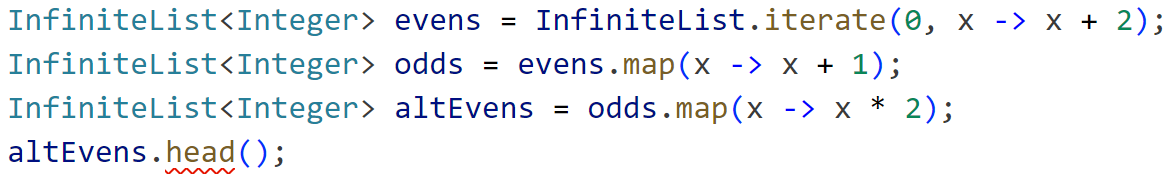
\includegraphics[width=1\linewidth]{Paper/Final/images/2.png} \\
    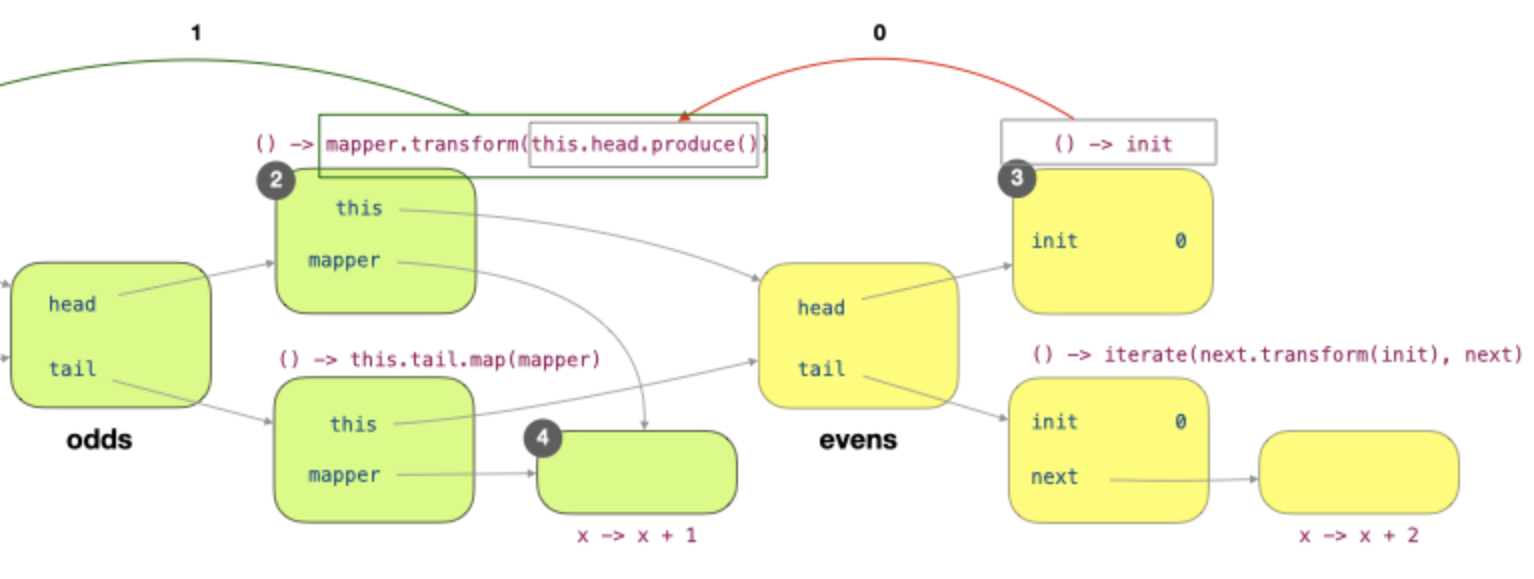
\includegraphics[width=1\linewidth]{Paper/Final/images/3.png} \\
    The \textbf{nested class }convention is shown as follows: \\
    \centerline{\includegraphics[width=1\linewidth]{Paper/Final/images/5.png}}
\end{enumerate}

\section{Functional Programming}
\begin{enumerate}
    \item \textbf{Pure Functions}
    \begin{itemize}
        \item No \textbf{side effects}: \textbf{No} 1) print to the screen, 2) write to files, 3) throw exceptions, 4) change other variables, 5) modify the values of the arguments
        \item \textbf{Deterministic}: Given the \textbf{same input} (can have \textbf{no input}), the function must produce the \textbf{same output}.
    \end{itemize}
    \item \textbf{Functional Interface}
    \begin{itemize}
        \item (\texttt{BooleanCondition<T>}):
        \begin{itemize}
            \item \textbf{Lambda example}: \texttt{BooleanCondition<Integer> isPositive = x -> x > 0;}
            \item \textbf{Java equivalent}: \texttt{Predicate<T>}.
        \end{itemize}
        \item (\texttt{Producer<T>}): 
        \begin{itemize}
            \item \textbf{Lambda example}: \texttt{Producer<Double> randomValue = () -> Math.random();}
            \item \textbf{Java equivalent}: \texttt{Supplier<T>}.
        \end{itemize}
        \item (\texttt{Consumer<T>}):
        \begin{itemize}
            \item \textbf{Lambda example}: \texttt{Consumer<String> printUpperCase = s -> System.out.println(s.toUpperCase());}
            \item \textbf{Java equivalent}: \texttt{Consumer<T>}
        \end{itemize}
        \item (\texttt{Transformer<U, T>}): Tranform a value of type \texttt{U} into a value of type \texttt{T}.
        \begin{itemize}
            \item \textbf{Lambda example}: \texttt{Transfomer<String, Integer> stringLength = s -> s.length();}
            \item \textbf{Java equivalent}: \texttt{Function<U,T>}
        \end{itemize}
        \item (\texttt{Combiner<S, T, R>}): Combine two values of type \texttt{S, T} into a value of type \texttt{S}.
        \begin{itemize}
            \item \textbf{Lambda example}: \texttt{Combiner<Integer, Integer, Integer> multiply = (a, b) -> a * b;}
            \item \textbf{Java equivalent}: \texttt{BiFunction<S, T, R>}.
        \end{itemize}
        \item \textbf{Tips}
        \begin{itemize}
            \item A \textbf{functional interface} must have \textbf{exactly one abstract method}, it \textbf{can have} any number of helpers (constants, static/default methods). It \textbf{can extend from another class}, but if the parent class has \textbf{multiple abstract method}, then the interface is \textbf{no longer a functional interface}.
            \item \textbf{All} the \textbf{fields} in an \textbf{interface} are \texttt{public static final} (constant) by default.
        \end{itemize}
    \end{itemize}
    \item \textbf{Method Referencing} \\
    \begin{itemize}
        \item \textbf{Steps to solve compile or not question}
        \begin{itemize}
            \item Determine \textbf{the number of inputs} according to the functional interface's \textbf{abstract method} (match with the number of parameters in this method), then your lambda will be like \texttt{(x, y, ..) -> ...}, the L.H.S is the number of inputs
            \item Use the rule to rewrite the normal lambda to see if 1) number of parameters matches 2) type matches (can find methods)
        \end{itemize}
        \item \textbf{Tips}: In \texttt{A::foo}, if \texttt{foo} is an \textbf{instance method}, it will use the first input as the instance, and pass the remaining inputs as arguments. Otherwise, it will call the \textbf{class method} and pass \textbf{all inputs as arguments}.
        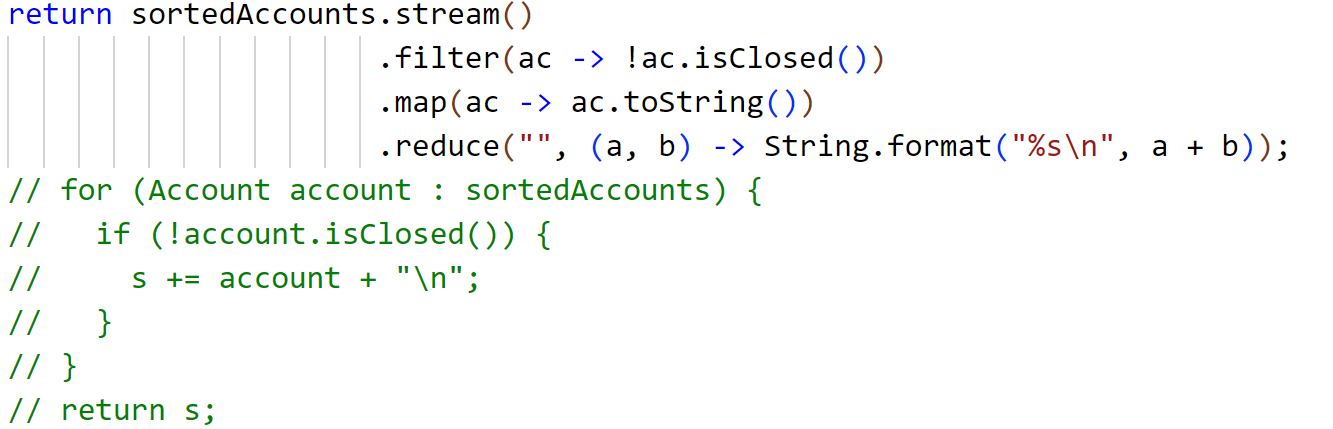
\includegraphics[width=1\linewidth]{Paper/Final/images/1.png}
    \end{itemize}
    \item \textbf{Curried Functions}: 1) Treat it as passing several parameters 2) treat it as a function that \textbf{returns another function}! e.g. \texttt{f -> x -> (f.apply(x + 0.01) - f.apply(x)) / 0.01;}.
    \item \textbf{Lambda Stack and Heap}: Notice that the local variables in \textbf{main} method will be captured! \\
    \centerline{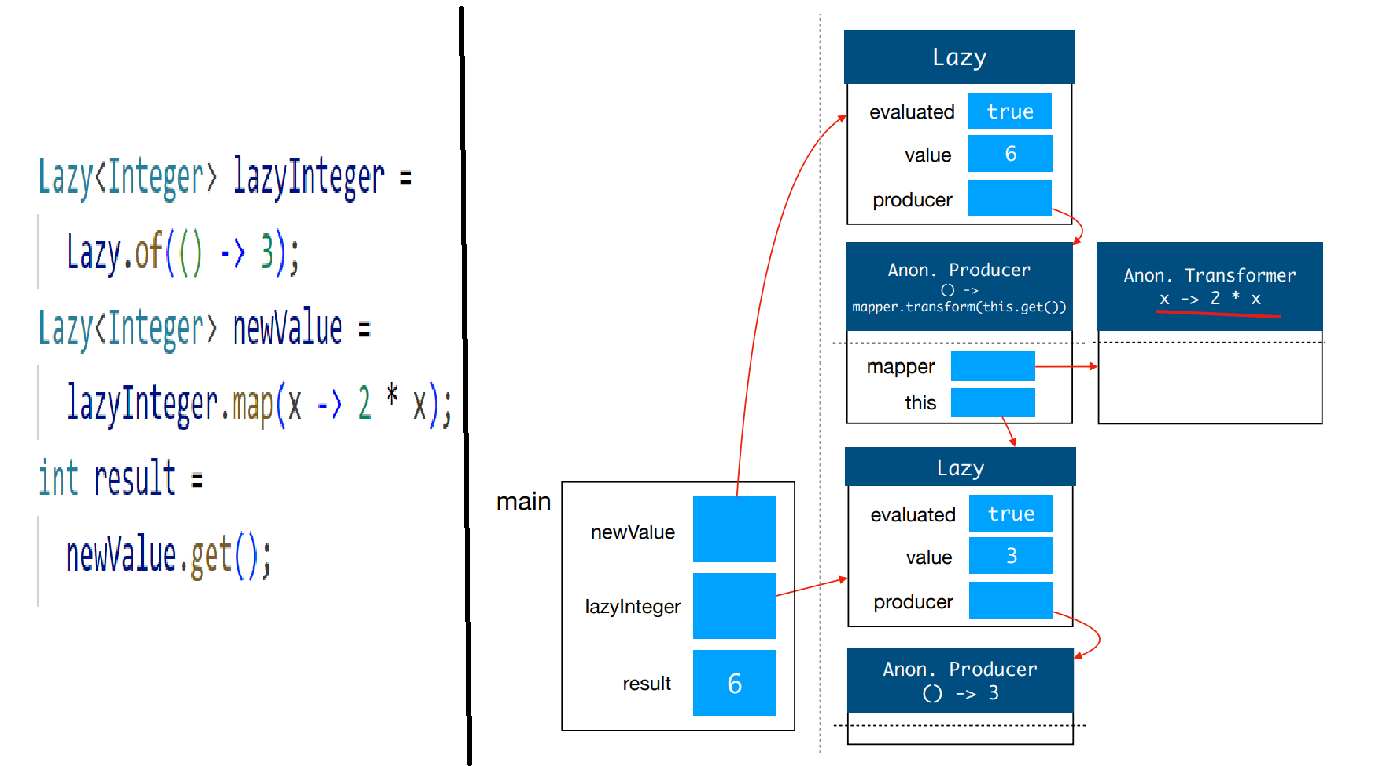
\includegraphics[width=1\linewidth]{Paper/Final/images/6.png}}
\end{enumerate}

\section{Stream}
\begin{enumerate}
    \item \textbf{reduce()}: Workflow is \textbf{result = identity} $\rightarrow$ \textbf{for each element in the stream; result = accumulator.apply(result, element); return result}
    \begin{itemize}
        \item \texttt{reduce(identity, accumulator)}: the \texttt{identity} and \texttt{element in the stream} must be of the \textbf{same} type!
        \item \texttt{reduce(identity, accumulator, combiner)}: the \textbf{identity} \textbf{may not be the same type} as the \textbf{element in the stream}. To use this safely and compatibly, must follow the \textbf{three rules}
        \begin{itemize}
            \item \textbf{Identity Rule}: \texttt{combiner.apply(identity, i) == i}
            \item \textbf{Associativity Rule}: \texttt{(x * y) * z == x * (y * z)} (\textbf{Both accumulator and combiner} should adhere to this rule)
            \item \textbf{Compatibility Rule}: \texttt{combiner.apply(u, accumulator.apply(identity, t)) == accumulator.apply(u, t)}
        \end{itemize}
    \end{itemize}
    \item \textbf{map()}: produce a new stream of the transformed elements with a \textbf{one-to-one relationship}. % \\
    % For example, here the \textbf{name} and the \textbf{cost after reducing} has a \textbf{one-to-one} relationship \\
    % \includegraphics[width=1.0\linewidth]{PE/PE2/images/5.png}
    \item \textbf{flatMap()}: transforms \textbf{each element} into a \textbf{stream} and then \textbf{flattens} all resulting streams into a single stream, useful for working \textbf{with nested collections} or \textbf{when one element should produce multiple output elements}. % \\
    % For example, here the \textbf{name} and the \textbf{cost} has a \textbf{one-to-multiple} relationship \\
    % \includegraphics[width=1.0\linewidth]{PE/PE2/images/4.png}
    \item \textbf{filter()}: Creates a new stream that keeps \textbf{only the elements that passed the test} in \texttt{Predicate}.
    \item \textbf{none/any/allMatch()}: a \textbf{boolean} method. It returns \texttt{true} only if \textbf{no/any/all} element in the stream \textbf{passes the predicate test}.
    \item \textbf{sorted()}: elements according to \textbf{natural order} (small to big or ascending order) or a \textbf{provided comparator}
    \item \textbf{Tips}
    \begin{itemize}
        \item \textbf{Times evaluted by calling \texttt{get(n)}} \\
        \begin{tabular}{|c|c|c|c|}
        \hline
        \textbf{generate} & \textbf{iterate} & \textbf{map} & \textbf{flatMap} \\
        \hline
        1                 & n                & 1             & 1               \\
        \hline
        \end{tabular}
        \item \texttt{sorted()} and \texttt{distinct()} are \textbf{stateful}, so should only be called on \textbf{finite streams}. Otherwise, enter infinite loop.
        \item \textbf{InfiniteList}: always use \texttt{head()} and \texttt{tail()}
        \begin{itemize}
            \item \texttt{head()}: return the \textbf{first non-filtered} element of the List.
            \item \texttt{tail()}: return the remaining list, excluding the \textbf{filtered-out} elements.
        \end{itemize}
    \end{itemize}
\end{enumerate}

\section{Monad and Functors}
\begin{enumerate}
    \item \textbf{Monad}: A class that can be created using \texttt{of} and chained using \texttt{flatMap}. And follows the three \textbf{Monad Laws}
    \item \textbf{Monad Laws}: These laws are used on \textbf{part of your lambda expression}
    \begin{itemize}
        \item \textbf{The Left Identity Law}: \texttt{Monad.of(x).flatMap(x -> f(x))} $\equiv$ \texttt{f(x)}. (The output of \texttt{f(x)} is by default a monad).
        \item \textbf{The Right Identity Law}: \texttt{monad.flatMap(x -> Monad.of(x))} $\equiv$ \texttt{monad}.
        \item \textbf{The Associative Law}: \texttt{monad.flatMap(x -> f(x)).flatMap(x -> g(x))} $\equiv$ \texttt{monad.flatMap(x -> f(x).flatMap(y -> g(y)))}
    \end{itemize}
    \item \textbf{Functor}: A class that has a \texttt{map} method and follows the two \textbf{Functor Laws}
    \item \textbf{Functor Laws}
    \begin{itemize}
        \item \textbf{Identity Law}: \texttt{functor.map(x -> x)} $\equiv$ \texttt{functor}.
        \item \textbf{Composition Law}: \texttt{functor.map(x -> f(x)).map(x -> g(x))} $\equiv$ \texttt{functor.map(x -> g(f(x))}.
    \end{itemize}
    \item \textbf{Tips}
    \begin{itemize}
        \item A class/type can be \textbf{both} monad and functor!
        \item Every \textbf{Monad is a Functor}, but \textbf{not every Functor is a Monad}.
        \item \textbf{Trace through the program step by step} to see if the certain class/type logic follows the three Monad Laws anot.\
        \item When using whatever monad/functor law, find the \textbf{part of the expression} that you are using that law, and replace it with the output of that law.
        \item To find the ultimate proof, try comparing \textbf{what you want} with \textbf{what you have} now. And then slowly slowly prove it.
    \end{itemize}
\end{enumerate}

\section{Parallel Stream}
\begin{enumerate}
    \item \textbf{Creation}: 1) call \texttt{.parallel()} on a \textbf{stream} or 2) call \texttt{.parallelStream()} on a \textbf{collection}.
    \item \textbf{After Creation}: The original stream is divided into several \textbf{substreams} or \textbf{threads} to run concurrently.
    \item \textbf{When can stream be parallelized}: The stream \textbf{should not have}
    \begin{itemize}
        \item an operation with a \textbf{side effect}
        \item an operation that \textbf{interferes with the stream data source.}
        \item an operation that is \textbf{stateful}, meaning depending on elements processed before, e.g. \texttt{sorted(), distinct(), limit()}
    \end{itemize}
    \item \textbf{Tips}
    \begin{itemize}
        \item \textbf{All parallel} programs are \textbf{concurrent}, but \textbf{not all concurrent} programs are \textbf{parallel}.
        \item Having \textbf{multiple cores/processors} is a \textbf{prerequisite} to running a program in \textbf{parallel}.
    \end{itemize}
\end{enumerate}

\section{Threads and CompletableFuture}
\begin{enumerate}
    \item \textbf{Threads}
    \begin{itemize}
        \item \textbf{Decide which Thread you are in}
        \begin{itemize}
            \item Find the position of the method call: \texttt{Thread.(whatever)}
            \item If it is \textbf{inside a lambda or Runnable} which is passed to \texttt{new Thread(...)}, you're in that \textbf{new thread}.
            \item If you're outside the \texttt{new Thread(...)}, e.g. in the \texttt{main} method, you're usually in the \texttt{main} thread.
        \end{itemize}
        \item \textbf{Pause a thread}: Done by calling \texttt{Thread.sleep(ms)}, it will pause the \textbf{thread you're in} (Use the method above to find out) for \textit{ms} seconds.
    \end{itemize}
    \item \textbf{CompletableFuture}
    \begin{itemize}
        \item \textbf{Rule of thumb}
        \begin{itemize}
            \item \texttt{CF(f).then(g)} means: \textbf{start} \texttt{g} \textbf{only after} \texttt{f} \textbf{has been completed}.
            \begin{itemize}
                \item Examples: \texttt{thenRun}, \texttt{thenCombine} -- combine, \texttt{thenApply} -- map, \texttt{thenCompose} -- flatMap, etc.
            \end{itemize}
            \item \texttt{static CF.async(g)} means: \textbf{start} \texttt{g} \textbf{on a new thread}
            \begin{itemize}
                \item Examples: \texttt{supplyAsync}, \texttt{runAsync}, etc.
            \end{itemize}
            \item \texttt{CF(f).then...async(g)} means: \textbf{start} \texttt{g} \textbf{only after} \texttt{f} \textbf{has been completed, but use a new thread.}
            \begin{itemize}
                \item Examples: \texttt{thenRunAsync}, \texttt{thenApplyAsync}, etc.
            \end{itemize}
            Difference between \texttt{run} and \texttt{supply}: \texttt{run} executes a \textbf{void function} while \texttt{supply} executes a \textbf{function with a return value}.
        \end{itemize} 
        \item \textbf{Creation}: 1) \texttt{completedFuture(value)}, 2) \texttt{runAsync(Runnable), supplyAsync(Supplier)} 3) Rely on other CompletableFutures, use \texttt{cf = anyOf(cfs)/allOf(cfs)}, which means the target \texttt{cf} will complete when \textbf{any/all} of the \texttt{cfs} complete.
        \item \textbf{Get the result}: 1) \texttt{get()}, will throw \textbf{checked exceptions} that must be handled 2) \texttt{join()}, will not and is \textbf{usually preferred}. These two methods are \textbf{synchronous calls}, will block the \textbf{main thread} until the \texttt{cf} finishes.
        \item \textbf{When is CompletableFuture complete}
        \begin{itemize}
            \item For \texttt{CompletableFuture<T> cf}:
                \begin{itemize}
                    \item \texttt{cf = CompletableFuture.supplyAsync(s)}: \textbf{complete} after \texttt{s.get()}
                    \item \texttt{cf = CompletableFuture.runAsync(r)}: \textbf{complete} after \texttt{r.run()}
                    \item Applies regardless of nested CompletableFutures in \texttt{s}/\texttt{r}
                \end{itemize}
            \item For \texttt{CompletableFuture<...> cf = CompletableFuture.completedFuture(f)}:
                \begin{itemize}
                    \item \textbf{complete} immediately after creation
                \end{itemize}
        \end{itemize}
    \end{itemize}
    \item \textbf{Tips}
    \begin{itemize}
        \item \texttt{System.out.println} is a \textbf{synchronous} method call!
        \item \textbf{Thread}: There is \textbf{no sequence} of which thread will be executed first. So, be always careful, there may be lots of possibilities!
        \item \textbf{CompletableFuture}: If \textbf{no} \texttt{.join()} or \texttt{.get()} is called after the CompletableFuture, the output may have \textbf{many possibilities}, a.k.a \textbf{non-determinstic output}.
        \item \textbf{CompletableFuture}: Possible output with \texttt{anyOf()} is a bit \textbf{tricky}, fully utilize your \textbf{exhaustive thinking}.
    \end{itemize}
\end{enumerate}

\section{Fork and Join}
\begin{enumerate}
    \item \textbf{Working Principles}
        \begin{itemize}
        \item Each thread has a deque of tasks.
        \item When a thread is idle, it checks its deque of tasks.
        \begin{itemize}
            \item If the deque is \textbf{not empty}, it picks up a task at the head of the deque to execute (e.g., invoke its \texttt{compute()} method).
            \item Otherwise, if the deque is \textbf{empty}, it picks up a task from the \textbf{\textit{tail}} of the deque of another thread to run. This is a mechanism called \textit{work stealing}.
        \end{itemize}
        \item When \texttt{fork()} is called, the caller (target) adds itself to the \textbf{\textit{head}} of the deque of \textbf{the executing thread}. This is done so that the most recently forked task gets executed next, similar to how normal recursive calls.
        \item When \texttt{join()} is called, several cases might happen.
        \begin{itemize}
            \item If the subtask (target, same for the follow) to be joined \textbf{hasn't been executed}, this subtask will be \textbf{popped out first}, and then its \texttt{compute()} method is called and the subtask is executed.
            \item If the subtask to be joined \textbf{has been completed} (some other thread has stolen this and completed it), then the result is read, and \texttt{join()} returns.
            \item If the subtask to be joined has been stolen and is being executed by another thread, then the current thread either finds some other tasks to work on from its \textbf{local deque}, or steals another task from \textbf{another deque}.
        \end{itemize}
    \end{itemize}
    \item \textbf{Tips}
    \begin{itemize}
        \item The \texttt{fork(), compute(), join()} order should form a \textbf{palindrome} and there should be \textbf{no crossing}. \\
        \centerline{\includegraphics[width=0.8\linewidth]{Paper/Final/images/4.png}}
        \item \texttt{task.compute()} is just a \textbf{normal method call}, this target \texttt{task} won't be added to the current worker's task dequeue.
        \item When dealing with \textbf{work stealing} problem, always write down the \textbf{content} of the worker to-be-stolen's \textbf{task dequeue}, and its \textbf{task at the tail} will be stolen!
    \end{itemize}
\end{enumerate}

\end{multicols}

\end{document}